\section{Definición de Integral}
La definición de la integral de Lebesgue posibilita extender la Integral de Riemann y establecer un cimiento sólido para todas aquellas áreas matemáticas que se nutren de la integración y que poseen situaciones peculiares que hacen las integrales de Riemann inservibles.

\begin{obs}
Recordemos que llamamos función simple a una función con la estructura:
$$\varphi = \sum_{k=1}^{m} \alpha_k \chi_{E_k}$$
Dicha función cumple que:
\begin{itemize}
    \item Es una función medible.
    \item Solo toma un número finito de valores.
    \item Cualquier función $\varphi$ que sea medible y solo tome un número finito de valores $(\beta_1, \ldots, \beta_r)$ es una función simple, puesto que podemos expresar dicha función como:
\begin{align*}
E_j = \varphi^{-1}\left(\{\beta_j\}\right) \text{, medible} & & \varphi = \sum_{k=1}^{r} \beta_j \chi_{E_j} \Rightarrow \varphi \text{ es simple.}
\end{align*}
\end{itemize}
\end{obs}

\begin{defi}[Integral]
Sea $\varphi$ función simple no negativa:
$$\varphi = \sum_{k=1}^{m} \alpha_k \cdot \chi_{E_k} \mbox{ donde } \left(\alpha_k > 0\right)$$
Definimos la \textbf{integral} de dicha función como:
$$I\left(\varphi\right) = \sum_{k=1}^{m} \alpha_k \mu\left(E_k\right)$$
\end{defi}

\begin{obs}
Como la medida de dichos conjuntos puede ser infinito y los valores $\alpha_k = 0$, es necesario que definamos $0 \cdot \left(+ \infty\right) = 0$ para poder dar una definición consistente de $I\left(\varphi\right) \in \left[0, +\infty\right]$.
\end{obs}


\begin{prop}
Sea $\varphi$ función simple, es posible escribir dicha función de distintas formas:
$$\varphi = \sum_{i=1}^{m} \alpha_i \chi_{E_i} = \sum_{i=1}^{p} \beta_i \chi_{D_i}$$
entonces la integral coincide para cualquiera que sea la forma escogida:
$$I(\varphi) = \sum_{i=1}^{m} \alpha_i \mu\left(E_i\right) = \sum_{i=1}^{p} \beta_i \mu\left(D_i\right)$$
luego la integral tiene una definición consistente.
\end{prop}
\begin{demo}
La demostración se deja como ejercicio de las hojas, se trata de utilizar que entre dos cualesquiera puedo pasar por la forma canónica y esta integral es la de la definición.
\end{demo}

\begin{prop}
\begin{enumerate}
    \item Sea $c > 0$ y $\varphi$ simple no negativa, entonces $I\left(c\cdot \varphi\right) = c\cdot I\left(\varphi\right)$.
    \item Sean $\varphi, \psi$ simples no negativas, entonces $I\left(\varphi + \psi\right) = I\left(\varphi\right) + I\left(\psi\right)$
    \item Si $\varphi \le \psi$ c.t.p, entonces $I\left(\varphi\right) \le I\left(\psi\right)$
    \item Si $\varphi = \psi$ c.t.p, entonces $I\left(\varphi\right) = I\left(\psi\right)$
\end{enumerate}
\end{prop}
\begin{obs}
Los conjuntos no tienen porque ser intervalos, si fuese este el caso sería, en el fondo, integrabilidad Riemann.
\end{obs}

\begin{prop}
Si $\varphi$ es una función simple no negativa y $A_1 \cap A_2 = \emptyset$:
\[
I \left( \varphi \left( x \right) \right) = I \left( \varphi \left( x \right) \cdot A_1 \right) + I \left( \varphi \left( x \right) \cdot A_2 \right)
\]
\end{prop}

\begin{defi}[Integral de Lebesgue]
Sea $f: \mathbb{R}^n \rightarrow \left[0, +\infty\right]$ una función medible, definimos la \textbf{integral de Lebesgue de $f$} de la siguiente\footnote{La definición no cambia si las funciones $\varphi \leq f$ en c.t.p.} forma:
$$\int_{\mathbb{R}^n}f \ d\mu = \sup_{\varphi \leq f} I\left(\varphi\right) \in \left[0, +\infty\right]$$
Donde las funciones $\varphi$ son simples no negativas.
\end{defi}

\begin{prop}
Sea $\varphi$ simple no negativa, la integral de Lebesgue coincide con la integral definida para este tipo de funciones:
$$\int_{\mathbb{R}^n}\varphi \ d \mu = I\left(\varphi\right)$$
\end{prop}
\begin{demo}
En primer lugar, la primera desigualdad la tenemos por ser el supremo de las Integrales de las funciones simples menores o iguales que $\varphi$, es decir:
$$\varphi \le \varphi \Rightarrow I\left(\varphi\right) \leq \sup_{\psi \leq \varphi} I(\psi) = \int_{\mathbb{R}^n} \varphi \ d \mu $$
Si $\int_{\mathbb{R}^n} \varphi \ d \mu = +\infty$, entonces tenemos que:
$$\forall M > 0,\ \exists \psi \le \varphi: I\left(\psi\right) \ge M \Rightarrow M \le I\left(\psi\right) \le I\left(\varphi\right) \Rightarrow \forall M > 0: I\left(\varphi\right) \ge M \Rightarrow I\left(\varphi\right) = +\infty$$
Si $\int_{\mathbb{R}^m}\varphi \ d \mu < +\infty$, entonces tenemos que:
$$\forall \varepsilon > 0,\ \exists \psi \le \varphi: I\left(\psi\right) \ge \int_{\mathbb{R}^n}\varphi \ d \mu - \varepsilon \Rightarrow I\left(\varphi\right) \ge I(\psi) \geq  \int_{\mathbb{R}^n}\varphi \ d \mu - \varepsilon \Rightarrow I\left(\varphi\right) \ge \int_{\mathbb{R}^n}\varphi \ d \mu$$
\end{demo}

\begin{prop}
Sean $f, g: \mathbb{R}^n \rightarrow \left[0, +\infty\right]$ dos funciones medibles tal que $f \le g$ c.t.p., entonces:
$$\int_{\mathbb{R}^n}f \ d \mu \le \int_{\mathbb{R}^n}g \ d \mu.$$
\end{prop}
\begin{demo}
Se deja como ejercicio.
\end{demo}

\begin{coro}
Sean $f, g: \mathbb{R}^n \rightarrow \left[0, +\infty\right]$ dos funciones medibles tal que $f = g$ c.t.p., entonces:
$$\int_{\mathbb{R}^n}f \ d \mu = \int_{\mathbb{R}^n} g \ d \mu$$
\end{coro}

\begin{defi}[Integral en un conjunto]
Sea $A \subset \mathbb{R}^n$ un conjunto medible y $f: A \rightarrow \left[0, +\infty\right]$ una función medible, entonces definimos \textbf{la integral de $f$ sobre $A$} como:
$$\int_A f \ d \mu = \int_{\mathbb{R}^n}f \cdot \chi_{A} \ d \mu$$
\end{defi}

\begin{obs}
En general se trabajará con funciones no infinitas para evitar que la integral sea infinita trivialmente.
\end{obs}

\begin{prop}
Si $f:\mathbb{R}^n\rightarrow \mathbb{R}$ es una función medible, entonces el conjunto $\{(x, f(x))\}$ que definimos como la gráfica $f$ tiene medida $0$.
\end{prop}

\begin{lema}
Sea $\varphi$ función simple no negativa y $\{A_k\}_{k=1}^{\infty}\uparrow A$ sucesión creciente $\left(A_k \subset A_{k+1} : \bigcup_{k \in \mathbb{N}} A_k = A\right)$ de conjuntos medibles convergentes a $A$, entonces:
$$\int_A \varphi \ d \mu = \lim_{k\rightarrow\infty} \int_{A_k} \varphi \ d \mu.$$
\end{lema}
\begin{demo}
Tenemos que $\varphi = \sum_{j=1}^{m} \alpha_j \cdot \chi_{E_j}$, entonces:
$$\lim_{k\rightarrow\infty} \int_{A_k} \varphi \ d \mu = \lim_{k\rightarrow\infty} \int_{\mathbb{R}^n}\varphi \cdot \chi_{A_k} \ d \mu =$$
$$= \lim_{k\rightarrow\infty} \int_{\mathbb{R}^n} \left(\sum_{j=1}^{m} \alpha_j \cdot \chi_{E_j}\cdot \chi_{A_k}\right) \ d \mu= \lim_{k\rightarrow\infty} \int_{\mathbb{R}^n} \left(\sum_{j=1}^{m} \alpha_j \cdot \chi_{E_j \cap A_k}\right) d \mu = $$
$$= \lim_{k\rightarrow\infty} \sum_{j=1}^{m} \left( \alpha_j \int_{\mathbb{R}^n} \chi_{E_j \cap A_k} d \mu \right) = \lim_{k\rightarrow\infty} \sum_{j=1}^{m} \alpha_j \cdot \mu\left(E_j \cap A_k\right) = \sum_{j=1}^{m} \alpha_j \cdot \lim_{k\rightarrow\infty} \mu\left(E_j \cap A_k\right) = $$
$$= \sum_{j=1}^{m} \alpha_j \cdot \mu\left(E_j \cap A\right) = \sum_{j=1}^{m} \left(\alpha_j \int_{\mathbb{R}^n} \chi_{E_j \cap A} \ d \mu\right) = \int_{\mathbb{R}^n}\sum_{j=1}^{m} \alpha_j \chi_{E_j} \chi_{A} \ d \mu= \int_{\mathbb{R}^n} \varphi \cdot \chi_A \ d \mu = \int_A \varphi \ d \mu$$
\end{demo}

\subsection{Propiedades de la integral}
Vamos a demostrar las operaciones y propiedades analíticas que tiene esta nueva definición de integral que se ha dado.

\begin{theo}[Convergencia Monótona]
Supongamos una sucesión creciente de funciones $\{f_k\}_{k=1}^\infty \uparrow f$ convergente\footnote{Esto quiere decir que $f_k \leq f_{k+1}$ y $\lim_{k\rightarrow\infty} f_k(x) = f(x)$ de forma puntual} a $f$ donde cada función $f_k: \mathbb{R}^n \rightarrow \left[0, +\infty\right]$ es medible, entonces:
$$\int_{\mathbb{R}^n}f \ d \mu = \lim_{k\rightarrow\infty} \int_{\mathbb{R}^n} f_k \ d \mu$$
El teorema también es válido si la convergencia es en c.t.p.
\end{theo}
\begin{demo}
Por la monotonía de la sucesión, tenemos que:
$$\forall k \in \mathbb{N}: f_k \le f \Rightarrow \int_{\mathbb{R}^n} f_k \ d \mu \le \int_{\mathbb{R}^n} f \ d \mu$$
Por tanto, tenemos asegurada la convergencia de la sucesión de integrales por ser acotada superiormente y creciente:
$$\left\lbrace \int_{\mathbb{R}^n} f_k \ d \mu \right\rbrace_{k=1}^{\infty}\uparrow \ \wedge \ \exists \lim_{k\rightarrow\infty} \int_{\mathbb{R}^n} f_k \ d \mu \le \int_{\mathbb{R}^n}f \ d \mu$$

Fijamos $\varphi \le f$ simple no negativa y un $c < 1$. De este modo, definimos la siguiente sucesión de conjuntos:
$$A_k = \{x \in \mathbb{R}^n: c\cdot \varphi\left(x\right) \leq f_k\left(x\right)\}$$
Dicho conjunto es medible para cada k por ser el conjunto de puntos donde una función vale más que 0.

Por ser creciente la sucesión de funciones, es decir, $f_k \le f_{k+1}$, entonces tenemos que:
$$A_k \subset A_{k+1} \Rightarrow \{A_k\}_{k=1}^{\infty} \uparrow \mathbb{R}^n \mbox{ ya que }\bigcup_{n\in \mathbb{N}}A_k = \mathbb{R}^n$$

Si $f(x) = \infty$, entonces tenemos que:
$$\lim_k f_k \left(x\right) = +\infty \Rightarrow c\cdot \varphi\left(x\right) \in \mathbb{R},\ \exists k \in \mathbb{N} : c\cdot \varphi\left(x\right) < f_k\left(x\right) \Rightarrow x \in A_k$$
Por otro lado, si tenemos que $0 < f\left(x\right) < \infty $, entonces:
$$\varphi\left(x\right) \le f\left(x\right) \Rightarrow c\cdot \varphi\left(x\right) < f\left(x\right) \Rightarrow \lim_{k\rightarrow\infty} f_k\left(x\right) = f\left(x\right) \Rightarrow \exists k \in \mathbb{N} : c\cdot \varphi\left(x\right) < f_k\left(x\right)\Rightarrow x\in A_k$$

Por tanto, por el lema anterior, al tener la sucesión creciente de los $A_k$, tenemos que:
$$c \cdot \int_{\mathbb{R}^n}\varphi \ d \mu = c\cdot \int_{\mathbb{R}^n \setminus \{x : f\left(x\right) = 0\}}\varphi \ d \mu = \int_{\mathbb{R}^n \setminus \{x : f\left(x\right) = 0\}} c  \cdot \varphi \ d \mu = $$
$$=\lim_{k\rightarrow\infty} \int_{A_k} c \cdot \varphi \ d \mu \le \lim_{k\rightarrow\infty} \int_{A_k} f_k \ d \mu \le \lim_{k\rightarrow\infty} \int_{\mathbb{R}^n} f_k \ d \mu$$
De este modo, como el $c$ es arbitrario, si se hace tender a $1$, tenemos que:
$$\int_{\mathbb{R}^n} \varphi \ d \mu \le \lim_{k\rightarrow\infty} \int_{\mathbb{R}^n} f_k \ d \mu \stackrel{\forall \varphi}{\Rightarrow} \int_{\mathbb{R}^n}f \ d \mu = \sup_{\varphi \le f} \int_{\mathbb{R}^n}\varphi \ d \mu \le \lim_{k\rightarrow\infty} \int_{\mathbb{R}^n}f_k \ d \mu$$
Y ya tendríamos demostradas las dos desigualdades.
\end{demo}

\begin{obs}
Este resultado sigue siendo cierto si se toman las hipótesis solo en c.t.p. Si ocurriese que $f_k \leq f$ no se cumpliera en un conjunto de medida nula, tomamos $f'_k$ que vale $f_k$ en todos los puntos donde se cumple y 0 en los que no. Como, por definición, $f_k = f'_k$ en c.t.p. la integral es la misma y la demostración no se ve alterada.
\end{obs}

\begin{theo}
Sea $f: \left[a, b\right] \rightarrow \mathbb{R}^+$ una función acotada e integrable Rienmann, entonces $f$ es integrable Lebesgue y verifica:
$$\int_{\left[a, b\right]}f \ d \mu = \int_a^b f\left(x\right)\ dx$$
\end{theo}
\begin{demo}
Por ser acotada, $\exists M > 0: f \le M\chi_{\left[a, b\right]}$, lo que implica que $\int f \ d \mu \leq \int M \cdot \chi_{[a,b]}$, es decir, que es integrable Lebesgue.

Además, por ser integrable Riemann, tenemos que:
$$\int_a^b f\left(x\right)dx = \sup_{P \in \wp} L\left(f, P\right) \Rightarrow \exists \{P_k\}_{k=1}^{\infty} : P_k \leq P_{k+1} : \int_a^b f\left(x\right) \ dx = \lim_{k\rightarrow \infty} L\left(f, P_k\right) = $$
$$= \lim_{k\rightarrow\infty} \sum_{S \in P_k} \inf \{f\left(x\right) : x \in S\}\mu\left(S\right) = \lim_{k\rightarrow\infty} \int_{\left[a, b\right]}\left(\underbrace{\sum m_S \left(f\right) \cdot \chi_S}_{\text{funcion simple}}\right) \ d \mu = $$
$$= \int_{\left[a, b\right]}\lim_{k\rightarrow\infty} f_k \ d \mu = \int_{\left[a, b\right]}f \ d \mu$$
Donde $f_k = \sum m_S\left(f\right) \chi_S$ y vemos que por ser crecientes las particiones que hemos tomado, dicha sucesión también lo es y por ello podemos aplicar el teorema.
\end{demo}

\begin{prop}
Sea $f: \mathbb{R}^n \rightarrow \mathbb{R}^n$ medible no negativa, entonces $\exists \{\varphi_k\}_{k=1}^{\infty}$ sucesión de funciones simples tal que $\{\varphi_k\}_{k=1}^\infty \uparrow f $ es creciente y converge \textbf{puntualmente}\footnote{Si la función $f$ es acotada, entonces la convergencia es \textbf{uniforme}} a $f$.
\end{prop}
\begin{demo}
Dividimos la imagen de la función en intervalos disjuntos $I_j = [(j-1) \cdot 2^{-k}, j \cdot 2^{-k}]$ donde $j = 1, \ldots, k \cdot 2^k$ y la unión de todos los intervalos resulta el intervalo $[0,k)$
$$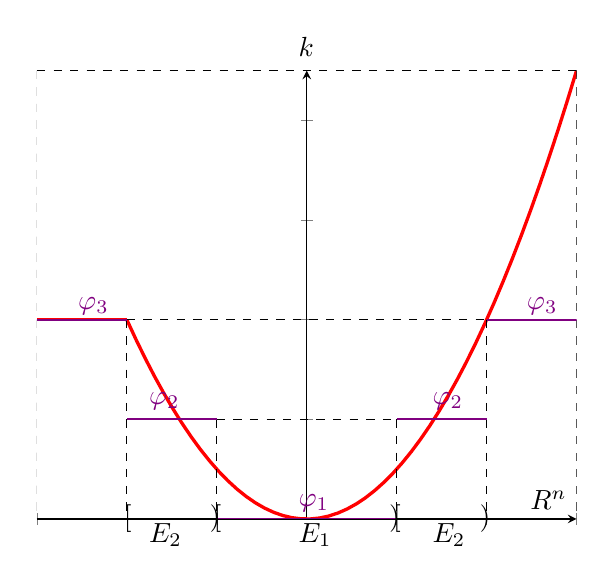
\begin{tikzpicture}
\begin{axis}[
axis y line=middle,
axis x line=middle,
xlabel=$\mathbb{R}^n$,
%grid = both, %major/minor
xticklabels={},yticklabels={}
];
\addplot [
very thick,red,mark=none,
domain=-2:3,samples=50,
] {(x^2)};
\addplot [
very thick,red,mark=none,
domain=-3:-2,samples=50,
] {4};
\draw [dashed] (-1,2) -- (1,2);
\draw [dashed] (-2,4) -- (2,4);
\draw [dashed] (-3,9) -- (3,9);

 \draw [dashed] (-1,2) -- (-1,0);
 \draw [dashed] (1,2) -- (1,0);
\draw [dashed] (-2,4) -- (-2,0);
\draw [dashed] (-3,9) -- (-3,0);
\draw [dashed] (2,4) -- (2,0);
\draw [dashed] (3,9) -- (3,0);

\draw[violet,  thick] (-1,0) -- (1,0);
\draw[violet,  thick] (-1,2) -- (-2,2);
\draw[violet,  thick] (1,2) -- (2,2);
\draw[violet,  thick] (2,4) -- (3,4);
\draw[violet,  thick] (-2,4) -- (-3,4);
   
\end{axis}

\node[color=black,right] at (3.2,-0.2) {$E_1$};
\node[color=black,right] at (1.3,-0.2) {$E_2$};
\node[color=black,right] at (4.9,-0.2) {$E_2$};
\node[color=black,right] at (3.2,6) {$k$};

\node[color=black,right] at (2.12,0) {$[$};
\node[color=black,right] at (2.07,0) {$)$};
\node[color=black,right] at (0.98,0) {$[$};
\node[color=black,right] at (4.35,0) {$)$};
\node[color=black,right] at (4.4,0) {$[$};
\node[color=black,right] at (5.5,0) {$)$};

\node[color=violet,right] at (3.2,0.2) {$\varphi_1$};
\node[color=violet,right] at (1.3,1.5) {$\varphi_2$};
\node[color=violet,right] at (4.9,1.5) {$\varphi_2$};
\node[color=violet,right] at (0.4,2.7) {$\varphi_3$};
\node[color=violet,right] at (6.1,2.7) {$\varphi_3$};
\end{tikzpicture}$$
Fijado un entero $k> 0$, definimos los siguientes conjuntos:
$$E_j^k := f^{-1}\left([(j-1)\cdot 2^{-k}, j\cdot 2^{-k} )\right)$$
Con dicha definición, es sencillo ver que los conjuntos son medibles, disjuntos y su unión queda como
$$\bigcup_{j=1}^{k\cdot 2^k}E_j^k = \{x\in  \mathbb{R}^n: f(x) < k\}$$
Definimos la siguiente función simple:
$$\varphi_k := \sum_{j=1}^{k\cdot 2^k} \frac{j-1}{2^k} \chi_{E_j^k}$$
Esto genera una sucesión de funciones creciente que denotamos por $\{\varphi_k\}_{k=1}^\infty \uparrow$.

Luego, por la definición que se ha dado de los $E_j^k$, dado $x \in \mathbb{R}^n,\ \exists k\in \mathbb{N} : \forall k \ge k_0: k > f\left(x\right) \Rightarrow x \in E_j^k$ para algún $j $ y, por tanto:
$$0 < f\left(x \right) - \varphi_k \left(x\right) < \frac{1}{2^k},\ \lim_{k \rightarrow \infty} \varphi_k\left(x\right) = f\left(x\right) $$
\end{demo}

\begin{prop}
Si $f, g: \mathbb{R}^n \rightarrow \mathbb{R}$ son funciones medibles no negativas, entonces la integral es aditiva, es decir:
$$\int_{\mathbb{R}^n} \left(f + g\right) \dif{\mu} = \int_{\mathbb{R}^n} f \dif{\mu} + \int_{\mathbb{R}^n} g \dif{\mu}$$
\end{prop}
\begin{demo}
Por la proposición anterior, existen dos sucesiones $\{\varphi_k\}_{k=1}^\infty$ y $\{\psi_k\}_{k=1}^\infty$ convergentes a $f$ y a $g$ respectivamente. De este modo, es trivial comprobar que $\{\varphi_k + \psi_k\}_{k=1}^\infty$ converge a $f+g$ y por el Teorema de Convergencia Monótona, tenemos que
$$\int_{\mathbb{R}^n}(f+g) \dif{\mu} = \lim_{k\rightarrow\infty} \int_{\mathbb{R}^n}(\varphi_k + \psi_k) \dif{\mu} = \lim_{k \rightarrow \infty} \left( \int_{\mathbb{R}^n} \varphi_k \dif{\mu} + \int_{\mathbb{R}^n} \psi \dif{\mu} \right) = \int_{\mathbb{R}^n} f \dif{\mu} + \int_{\mathbb{R}^n} g \dif{\mu}$$
\end{demo}

\begin{prop}
Sea $f: \mathbb{R}^n \rightarrow \mathbb{R}$ una función medible no negativa y $c\in \mathbb{R}^+$, entonces: 
$$\int_{\mathbb{R}^n} \left(c f\right) \dif{\mu} = c \int_{\mathbb{R}^n}f \dif{\mu}$$
\end{prop}
\begin{demo}
Completamente análoga a la anterior y se deja como ejercicio.
\end{demo}

\begin{theo}[Convergencia monótona para series]
Sea $\{f_k\}_{n=1}^{\infty}$ una sucesión de funciones medibles no negativas, entonces: 
$$\int_{\mathbb{R}^n} \left(\sum_{k=1}^{\infty} f_k \right) \dif{\mu} = \sum_{k=1}^{\infty}\left( \int_{\mathbb{R}^n} f_k \dif{\mu}\right)$$
\end{theo}
\begin{demo}
La demostración es prácticamente consecuencia de los enunciados anteriores:
$$\int_{\mathbb{R}^n} \left(\sum_{k=1}^{\infty} f_k\right) \dif{\mu} = \int_{\mathbb{R}^n} \lim_{m \rightarrow \infty} \left(\sum_{k=1}^{m} f_k \right)\dif{\mu} = \lim_{m \rightarrow \infty}\int_{\mathbb{R}^n} \left(\sum_{k=1}^{m} f_k\right) \dif{\mu} = $$
$$=\lim_{m \rightarrow \infty} \sum_{k=1}^{m} \left(\int_{\mathbb{R}^n} f_k \dif{\mu}\right) = \sum_{k=1}^{\infty} \left(\int_{\mathbb{R}^n} f_k \dif{\mu}\right) $$
\end{demo}

\begin{lema}[de Fatou]
Sea $\{f_k\}_{k=1}^{\infty}$ una sucesión de funciones medibles no negativas, entonces: 
$$\int_{\mathbb{R}^n} \left( \liminf_{k \rightarrow \infty}f_k \right) \dif{\mu} \le \liminf_{k \rightarrow \infty} \left(\int_{\mathbb{R}^n} f_k \dif{\mu}\right) $$
\end{lema}
\begin{demo}
Definimos las funciones $g_k = \inf_{m \ge k} f_m \ge 0$ medibles de modo que estas forman una sucesión creciente $\{g_k\}_{k=1}^\infty\uparrow$. En consecuencia, basta ver que:
$$\int_{\mathbb{R}^n} \left(\liminf_{k \rightarrow \infty}f_k \right) \dif{\mu} = \int_{\mathbb{R}^n} \left(\lim_{k \rightarrow \infty}g_k \right)\dif{\mu} =  \lim_{k \rightarrow \infty} \int_{\mathbb{R}^n} g_k \dif{\mu} = \liminf_{k \rightarrow \infty}\int_{\mathbb{R}^n} g_k \dif{\mu} \le \liminf_{k \rightarrow \infty} \int_{\mathbb{R}^n} f_k \dif{\mu}$$
\end{demo}

\begin{prop}
Las integrales impropias se soportan por la integral de Lebesgue:
\begin{align*}
\int_a^\infty f(x) \dif{x} = \int_{[a, \infty)}f(x)\dif{\mu} & &\int_a^b f(x)\dif{x} = \int_{[a,b]} f(x) \dif{\mu}
\end{align*}
\end{prop}
\begin{demo}
\begin{itemize}
\item Primera
$$\int_a^{\infty} f \left(x\right) dx = \lim_{M \rightarrow \infty} \int_a^M f \left(x\right) dx = \lim_{m \rightarrow \infty} \int_a^{\infty} f \left(x\right) \chi_{\left[a, M\right]}dx = \lim_{m \rightarrow \infty} \int_{\left[a, +\infty\right]} f \chi_{\left[a, M\right]} d \mu =$$
$$= \int_{\left[a, +\infty\right]} f \chi_{\left[a, +\infty\right]} d \mu = \int_{\left[a, +\infty\right]} f d \mu. $$
\item Segunda
$$\int_a^b f \left(x\right) dx = \lim_{k \rightarrow \infty}\int_a^{b - \frac{1}{k}} f \left(x\right) dx = \lim_{k \rightarrow \infty} \int_{\left[a, b - \frac{1}{k}\right]} f d \mu =$$
$$= \lim_{k \rightarrow \infty} \int_{\mathbb{R}} f \chi_{\left[a, b - \frac{1}{k}\right]} d \mu = \int_{\mathbb{R}} f \chi_{\left[a, b\right]} d \mu = \int_{\left[a, b\right]} f d \mu.$$
\end{itemize}
\end{demo}
